\newpage            
	\subsection{Aplikacja mobilna}
	Aplikację mobilną napisałem z myślą o uruchamianiu jej w systemie operacyjnym Android. Jest to system operacyjny na urządzenia mobilne oparty na zmodyfikowanym jądrze systemu operacyjnego Linux, 
	rozwijany przez sojusz biznesowy Open Handset Alliance~\cite{OHA}. Android tworzony jest w modelu otwartego oprogramowania, a źródłem jego finansowanie jest w znacznej mierze korporacja Google.
	Według danych firmy Statista, w styczniu 2022 r.\ Android był najpopularniejszym systemem operacyjnym na urządzenia mobilne, z niemal siedemdziesięcioprocentowym 
	udziałem w rynku tych urządzeń~\cite{OS_SHARE}. Jest on także wykorzystywany jako system operacyjny w przemyśle motoryzacyjnym (Android Auto), telewizyjnym (Android TV) oraz
	w urządzeniach mobilnych typu Smartwatch (Wear OS).

		\subsubsection{Kotlin i Android Studio}
		Aplikację mobilną napisałem w języku programowania Kotlin~\cite{KT_MAIN}. Jest to wieloplatformowy, statycznie typowany język programowania stworzony i rozwijany przez firmę JetBrains.
		Od 2019 roku jest on zalecany przez Google jako podstawowy język programowania na system operacyjny Android~\cite{ANDROID_KT}. Język ten jest zaprojektowany z myślą o
		pełnym współdziałaniu z językiem Java, poprzednikiem Kotlina jako głównego języka w programowaniu na Androida. Poza językiem Kotlin wykorzystany został także język znaczników XML, służący do projektowania warstwy graficznej aplikacji, oraz Gradle, narzędzie do automatyzacji budowania projektów, 
		wspierane jako oficjalny system budowania projektów na system Android. 

		Do napisania aplikacji wykorzystałem zintegrowane środowisko deweloperskie (ang.\ \emph{Integrated Development Envirnoment}, IDE) Android Studio~\cite{MEET_AS}. Jest to oficjalne IDE systemu operacyjnego
		Android stworzone we współpracy firm Google i JetBrains. Oferuje ono wiele narzędzi wspierających budowanie aplikacji na system Android. Android Studio zapewnia m.in.\@ inteligenty edytor kodu
		uzupełniający kod pisany w Kotlinie, Javie lub C/C++, graficzny edytor wspomagający tworzenie wizualnej części aplikacji, wbudowany, prosty w obsłudze emulator urządzenia mobilnego z 
		systemem Android, czy zintegrowany system budowania projektów Gradle. 

%\newpage
		\subsubsection{Model danych}
		W aplikacji wykorzystane są cztery klasy danych mające reprezentować obiekty umieszczane w bazie danych. 
		Są to: 

         \begin{itemize}
         	\item  \textsc{User} (Użytkownik) — jest to klasa zawierająca pseudonim użytkownika, jego unikalny identyfikator oraz adres e-mail. 
		
		\item \textsc{Place} (Miejsce) — najbardziej istotna klasa danych w aplikacji, reprezentująca miejsca dodawane na mapie przez użytkowników. Użytkownik dodający miejsce ma możliwość przypisania mu 
		Nazwy, Opisu, Kategorii (do wyboru z pięciu gotowych) oraz poziomu prywatności (miejsce prywatne nie będzie wyświetlane na mapie podczas wyszukiwania). Ponadto, każde Miejsce zawiera:
		unikalny identyfikator, długość i szerokość geograficzną (sczytane z położenia kursora w trakcie dodawania miejsca), GeoHash (typ danych, będący zaszyfrowanymi współrzędnymi geograficznymi miejsca, 
		mający usprawnić wydajność geograficznych zapytań do bazy danych~\cite{GEOHASH}), identyfikator i pseudonim autora miejsca, listę kategorii (ponieważ miejsce może należeć do więcej niż jednej 
		kategorii naraz), listę etykiet przypisanych miejscu przez wszystkich użytkowników, licznik polubień danego miejsca, listę identyfikatorów użytkowników, którzy polubili dane miejsce oraz flagę 
		definiującą jego prywatność. 
		
		\item \textsc{Tag} (Etykieta) — prosta klasa tworząca system etykiet. System ten inspirowany jest systemem etykiet wykorzystanym przez firmę Valve w platformie dystrybucji cyfrowej Steam.
		Jest to platforma, która łączy w sobie funkcje platformy dystrybucji programów komputerowych (głównie gier komputerowych i oprogramowania z nimi związanego) oraz serwisu społecznościowego.
		System etykiet stworzony przez Valve pozwala użytkownikom na dodawanie do znajdujących się w ofercie programów etykiet w postaci kilku słów np. ,,łamigłówki'', ,,trudna'', ,,gra z otwartym światem''.
		Znajdujących się w bazie danych etykiet można używać, aby filtrować wyniki wyszukiwania w ofercie platformy Steam~\cite{STEAM}. System znaczników obecny w aplikacji mobilnej, podobnie jak system
		Valve, pozwala każdemu użytkownikowi dodawać etykiety do każdego miejsca publicznego. Z uwagi na rozmiar projektu i ograniczenia techniczne, system ten nie umożliwia użytkownikom tworzenia nowych
		etykiet, a jedynie na korzystanie z gotowego zbioru etykiet prezentowanego w menu dodawania etykiet. Klasa etykiety składa się z nazwy etykiety, licznika dodań oraz listy użytkowników, którzy
		dodali etykietę do miejsca. W menu wyświetlającym szczegóły miejsca znajduje się lista wyświetlająca najpopularniejsze etykiety. Każdy użytkownik może dodać konkretną etykietę tylko raz, a 
		w bazie danych zliczane jest, ile razy dana etykieta została dodana do danego miejsca. To pozwala na wyświetlenie (w menu przedstawiającym szczegóły miejsca) dziesięciu najpopularniejszych etykiet
		danego miejsca. Pozwala to użytkownikom na określanie tego, jakie aktywności można w danym miejscu wykonywać, np. ,,muzeum'', ,,pomnik'', ,,bar'', ,,kino'' itp. Najpopularniejsze etykiety powinny najlepiej
		reprezentować przeznaczenie danego miejsca.
\newpage
		\item \textsc{Trip} (Wycieczka) — jest to klasa reprezentująca zbiór miejsc, wykorzystywana do tworzenia zapytań o trasę w Directions API.\@ Użytkownik tworzący wycieczkę
		może ustalić jej nazwę, opis i prywatność, a następnie dodawać do niej miejsca. Każda wycieczka może zawierać w sobie do 10 miejsc — ograniczenie to wprowadziłem, biorąc pod uwagę koszt odpowiedzi na bardziej złożone zapytania
		w Directions API.\@ Oprócz pól ustalanych przez użytkownika wycieczka zawiera także unikalny identyfikator, identyfikator i pseudonim autora, licznik polubień  oraz listę identyfikatorów 
		użytkowników, którzy polubili daną wycieczkę. 
     \end{itemize}
		
		Szczegółową reprezentację klas danych oraz zachodzących pomiędzy nimi relacji przedstawia poniższy diagram (Rysunek~\ref{relations}).

		\vspace{1cm}
        \begin{figure}[!ht]%
            \centering
            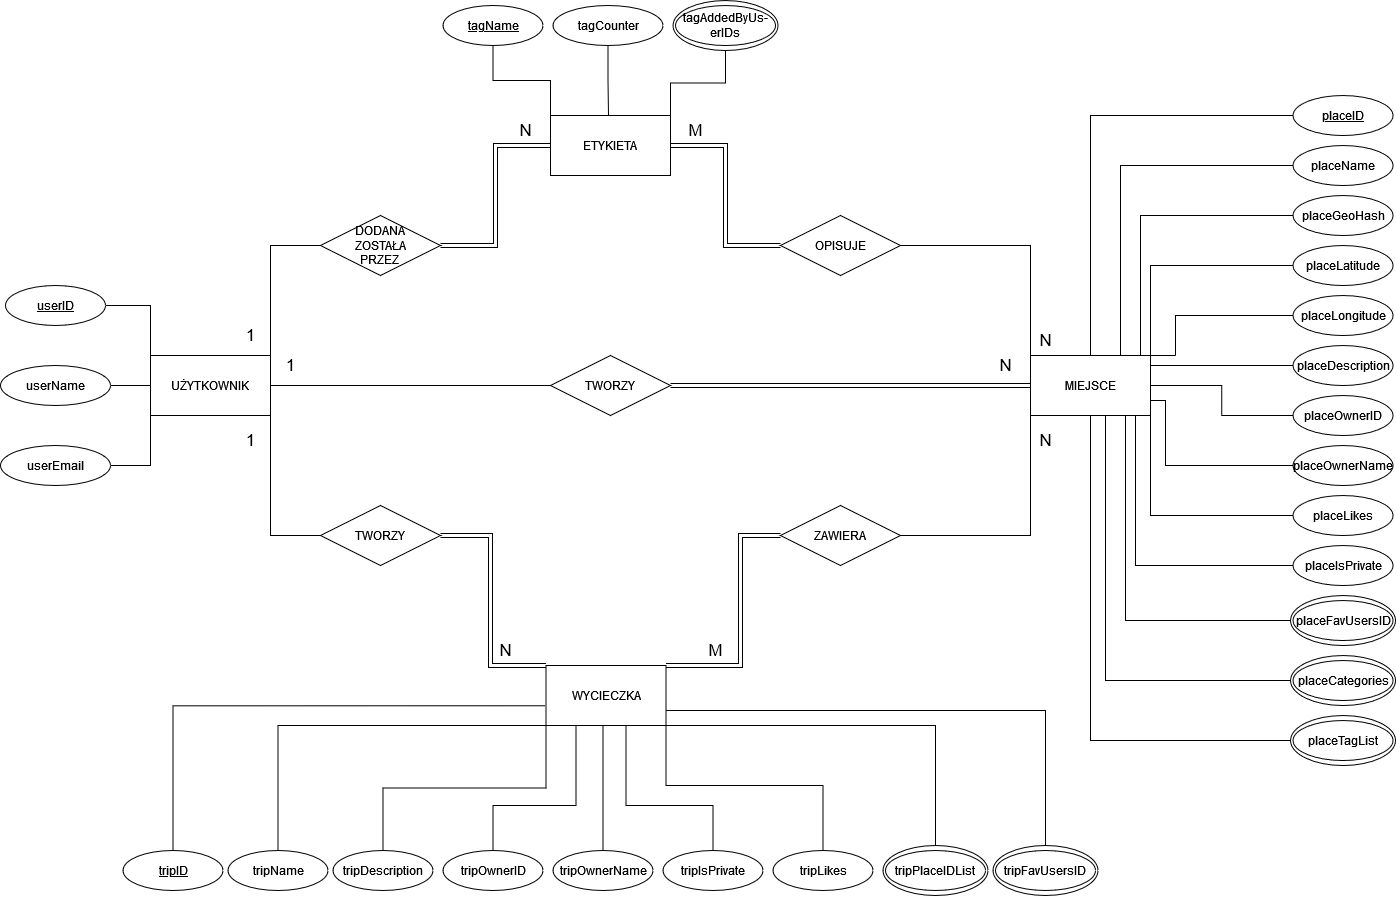
\includegraphics[scale=0.34]{src/relations_diagram.png}
            \caption{Schemat relacji w bazie danych mojej aplikacji.\label{relations}}
            \qquad
        \end{figure} 


